\section{Modelo de Actividad}
En la literatura la mayor\'ia de modelos contextuales comparten elementos que comunmente describen cuatro factores t\'ipicos de contexto \cite{abowd1999towards}: ubicaci\'on, identidad, estado de las personas, grupos y objetos f\'isicos y virtuales. Algunos de estos modelos difieren en la forma de ser representados, o en el \'ambito en el que se aplican, desde representaci\'ones de espacios de trabajo \cite{decouchant2013adapting}, meta modelos que describen el comportamiento de un grupo de usuarios \cite{montane2013context} \cite{alves2013radiator} \cite{hoyos2013domain}, hasta aquellos modelos enfocados a las actividades de un usuario y su comportamiento \cite{kamoun2012fadyrcos}\cite{gallardo2012framework}\cite{guermah2013ontology}\cite{Doweling2012ATheory}. Para el presente trabajo se hace uso de un meta modelo contextual para el modelado de sistemas groupware basado un modelo propuesto anteriormente\cite{montane2013context}, en el cual se pueden encontrar dos categor\'ias de elementos, interactivos y cohesivos.  Entre los interactivos se encuentran \textit{actores}, que son los usuarios del sistema, \textit{objetos} que se usan en \textit{tareas} o que son producto de ellas, \textit{categor\'ias} que clasifican a los actores, objetos y tareas seg\'un sus atributos, por \'ultimo est\'an los roles del objeto y del actor los cuales son asignadas a una tarea para establecer el rol que va a tener el actor u objeto involucrado en dicha tarea. Entre los datos cohesivos se encuentran las \textit{comunidades} que son el conjunto de actores con una \textit{actividad} en com\'un, estas actividades pueden tener varias \textit{metas} las cuales se cumplen realizando tareas. Por \'ultimo se encuentran las reglas que son sentencias en un lenguaje definido para poder inferir las interacciones que suceden en el groupware. En la figura \ref{cmp:mmc} se muestra un diagrama de los elementos de este modelo y sus relaciones.

\begin{figure}[h!]
  \centering
    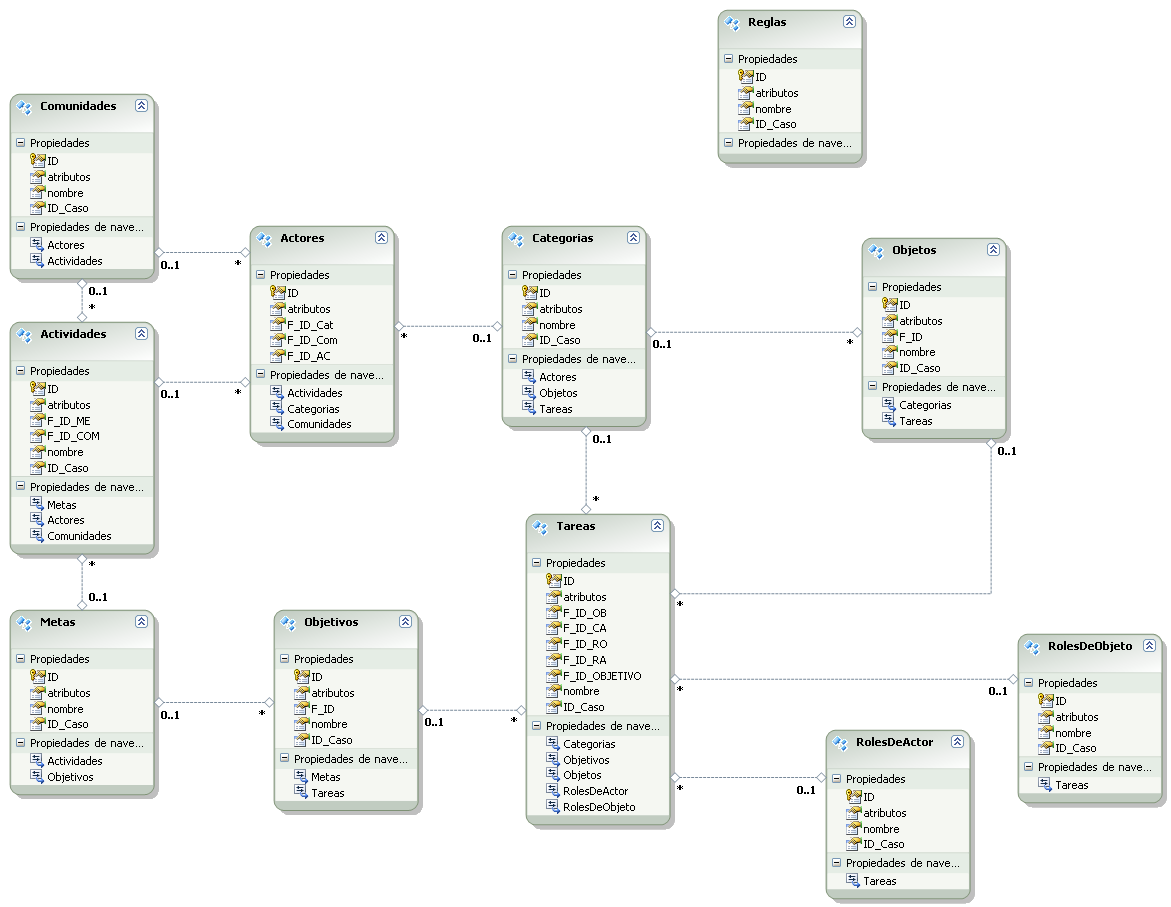
\includegraphics[scale=0.35]{images/modelo}
  \caption{Meta modelo contextual}
  \label{cmp:mmc}
\end{figure}

Con este meta modelo contextual se pueden describir groupwares definiendo cada uno de estos elementos a partir de interacciones, una vez dado de alta un caso junto con sus reglas se instancia un modelo que representar\'a al sistema colaborativo y almacenar\'a las variables contextuales que este transmita a la arquitectura. Cabe mencionar que en este metamodelo los elementos cuentan con 3 atributos principales, un identificador del objeto, un nombre descriptivo, y una lista de atributos almacenados en formato JSON, lo que vuelve flexible la forma de registrar casos de estudio.